% !TEX TS-program = pdflatex
% !TeX program = pdflatex
% !TEX encoding = UTF-8
% !TEX spellcheck = fr

\documentclass[11pt, a4paper]{article}
%\usepackage{fullpage}
\usepackage[left=1cm,right=1cm,top=1cm,bottom=2cm]{geometry}
\usepackage[fleqn]{amsmath}
\usepackage{amssymb}
%\usepackage{indentfirst}
\usepackage[T1]{fontenc}
\usepackage[utf8]{inputenc}
\usepackage[french,english]{babel}
\usepackage{txfonts} 
\usepackage[]{graphicx}
\usepackage{multirow}
\usepackage{hyperref}
\usepackage{parskip}
\usepackage{multicol}
\usepackage{wrapfig}

\usepackage{turnstile}%Induction symbole

\usepackage{tikz}
\usetikzlibrary{arrows, automata}
\usetikzlibrary{decorations.pathmorphing}

\renewcommand{\baselinestretch}{1}

\setlength{\parindent}{24pt}


\begin{document}

\selectlanguage {french}
%\pagestyle{empty} 

\noindent
\begin{tabular}{ll}
\multirow{3}{*}{\includegraphics[width=1.5cm]{../extra/logo/esi.ml.pdf}} & \'Ecole national Supérieure d'Informatique\\
& 2\textsuperscript{ème} année cycle supérieure (2CSSIL2, 2CSSIQ2)\\
& Machine Learning (2022-2023)
\end{tabular}\\[.25cm]
\noindent\rule{\textwidth}{1pt}\\%[-0.25cm]
\begin{center}
{\LARGE \textbf{Workshop: Réseaux de neurones avanc\'es (Autoencodeur \& CNN))}}
\begin{flushright}
	ARIES Abdelkrime
\end{flushright}
\end{center}
\noindent\rule{\textwidth}{1pt}

\section*{Information}

\begin{itemize}
	\item \textbf{APIs} : tensorflow, scikit-learn, numpy, jupyter notebook, pandas, matplotlib
	\item \textbf{Datasets} : Pokemon Image Dataset : {\scriptsize\url{https://www.kaggle.com/datasets/vishalsubbiah/pokemon-images-and-types}}
	\item \textbf{Documentation}: Tutoriel ({\scriptsize \url{https://github.com/projeduc/ESI_ML/tree/main/demos/NN}}), Tensorflow ({\scriptsize \url{https://www.tensorflow.org/api_docs/python/tf/}})
	\item \textbf{Pré-traitement} : Fourni avec ce workshop (il faut renommer le dossier comme "pokemon" ou changer le chemin du dataset dans le code fourni)
\end{itemize}

\section{Classement CNN}

\begin{itemize}
	\item Concevoir un modèle qui classe les pokémons selon leurs types (voir la figure \ref{fig:CNN-pok-cls}).
	\item Entraîner le modèle avec validation en calculant l'accuracy.
	\item Dessiner l'évolution des coûts (entrainement et validation).
	\item Calculer la précision et rappel sur le dataset de test.
	\item Proposer une autre architecture pour améliorer la performance en terme de précision et rappel.
\end{itemize}

\begin{figure}[htp]
	\centering
	\includegraphics[width=0.8\textwidth]{../img/workshop/CNN-pok-cls.pdf}
	\caption{Architecture de classement Pokemon basée sur les CNN.}
	\label{fig:CNN-pok-cls}
\end{figure}

\section{Auto-encodeur de clustering}

\begin{itemize}
	\item Concevoir le modèle illustré dans la figure \ref{fig:MLP-pok-cluster}. Ensuite, un autre CNN.
	La définition du modèle doit être re-utilisable ; c-a-d. elle doit être définie pour n'importe quelle taille d'image et du code (voir la figure \ref{fig:pok-cluster-CD}).
	Voici la description de quelques méthodes :  
	\begin{itemize}
		\item \textbf{\_\_init\_\_} : Prend comme paramètres la taille du code et la forme d'entre\'e \textbf{in\_shape}.
		Elle définit les couches de l'encodeur et le décodeur de la figure \ref{fig:CNN-pok-cls}.
		Pour que \textbf{model.summary()} fonctionne, nous devons créer le graphe. Donc, ajouter ce code après la définition des couches
		\begin{verbatim}
			inimg = Input(shape=in_shape)
			super().__init__(inimg, self.call(inimg))
		\end{verbatim}
		\item \textbf{encoder} : Prend une image comme paramètre et génère un code.
		\item \textbf{decoder} : Prend un code comme paramètre et génère une image.
		\item \textbf{call} : Une redéfinition de la méthode de la super-classe. 
		Elle a comme entrée une image et en sortie la reconstruction de l'image.
		\item \textbf{train\_step}: Prend un batch des images, applique une propagation en avant et une retro-propagation.
		\begin{verbatim}
			def train_step(self, data):
			    with tf.GradientTape() as tape:
			        img_pred = self.call(data)
			        loss = self.loss(data, img_pred)

			    variables = self.trainable_variables 
			    gradients = tape.gradient(loss, variables)
			    self.optimizer.apply_gradients(zip(gradients, variables))

			    return {'loss': loss}
		\end{verbatim}
	\end{itemize}
	\item Créer un modèle avec un code de 2. 
	Compiler le modèle et entrainer le avec Adam comme optimiseur et MSE comme fonction du cout.
	\item Générer les codes des Pokemons d'entrainement.
	\item Ploter leurs positions en se basant sur ce code en indiquant leurs types (couleur).
	\item Apparemment un vecteur de 2 n'est pas aussi suffisant pour représenter les différences. 
	Donc, essayer d'entrainer un autre modèle avec un code de 10 éléments. Générer les codes d'entrainement pour être utilis\'es pour le clustering.
	\item Appliquer K-Means sur les Pokemons d'entrainement en se basant sur leurs codes. 
	Ici, K est le nombre des classes.
	\item Pour chaque cluster généré, nous supposons que la classe majoritaire est celle représentée par ce cluster.
	\item Calculer l'indice de Rand : \textbf{sklearn.metrics.rand\_score}
	\item Répéter la même chose avec l'auto-encodeur CNN.
\end{itemize}

\begin{figure}[htp]
	\centering
	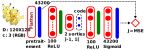
\includegraphics[width=0.6\textwidth]{../img/workshop/MLP-pok-cluster.pdf}
	\caption{Architecture Auto-encodeur clusterer des Pokemons en utilisant un MLP.}
	\label{fig:MLP-pok-cluster}
\end{figure}

\begin{figure}[htp]
	\centering
	\includegraphics[width=0.6\textwidth]{../img/workshop/pok-cluster-classD.png}
	\caption{Diagramme de classes des deux auto-encodeurs.}
	\label{fig:pok-cluster-CD}
\end{figure}


\section{Auto-encodeur de clustering pour classement}

Concevoir un modèle qui prend le code généré par l'auto-encodeur précédent et classe le pokémon selon son type : 
\begin{itemize}
	\item Il faut utiliser l'encodeur entraîné précédemment ; c-à-d. l'entrée doit être une image et pas le vecteur de son code. 
	Ensuite, l'auto-encodeur encode l'image en utilisant la méthode \textbf{encoder}.
	\item Le modèle de classement est un MLP (obviously!) qui prend la sortie de l'encodeur comme entrée et qui génère le type du pokémon.
	\item Lors de l'entraînement du classeur, il ne faut pas mettre à jours l'encodeur ; il faut désactiver l'entraînement du modèle : \textbf{model.trainable = False}.
	\item Comparer ce modèle avec celui du classement (première section).
\end{itemize}

\section{Génération des images}

Nous voulons concevoir un modèle qui génère des nouveaux pokémons en suivant les spécifications suivantes : 
\begin{itemize}
	\item Le code est un vecteur de 10 éléments.
	\item Utiliser des CNNs afin de minimiser le nombre des paramètres.
	\item En plus de la variable latente, nous devons utiliser un vecteur qui représente le type, afin d'apprendre \'a générer un pokémon selon le type.
\end{itemize}

Pour ce faire, nous allons utiliser deux approches :
\begin{itemize}
	\item \textbf{Autoencodeur variationnel} : 
	\begin{itemize}
		\item Similaire \'a \textbf{ClusterCNNAE}, mais qui a comme entrée au décodeur 3 vecteurs comme indiqué dans la figure \ref{fig:gen}(a).
	\end{itemize}
	\item \textbf{GAN} : 
	\begin{itemize}
		\item Voir la figure \ref{fig:gen}(b). Un GAN se compose de deux éléments : un générateur et un discriminateur. 
		Ce dernier a comme but de classer les images comme réelles ou triquées (classement binaire). 
		Le GAN a comme but de triquer le discriminateur (il doit générer des images tellement réelles, le discriminateur ne peut pas les détecter).
		\item Nous avons M images réelles. 
		Pour chaque itération, nous générons M images avec le générateur. 
		Nous passons les 2M images par le discriminateur et nous calculons l'erreur avec réelles (1) et générées (0).
		L'erreur est utilisée pour mettre \'a jours les paramètres du discriminateur.
		Ensuite, nous générons M images avec le générateur. 
		Ces images sont passées par le discriminateur afin de calculer l'erreur, mais avec un label = 1 (ici, l'erreur est calculée en supposant que le discriminateur considère les images comme réelles).
		Cette erreur sera utilisée pour mettre \'a jours les paramètres du générateur.
		\item En tensorflow, nous ne pouvons pas injecter l'erreur directement \'a la fin d'un modèle ; il faut définir une fonction d'erreur en se basant sur ses sorties.
		Dans ce cas, nous supposons que l'erreur de chaque sortie du générateur $S_i$ o\'u $S[32, 32, 3]$ est calculée en se basant sur l'erreur du discriminateur $J_D$ comme suit :
		\[\frac{\partial J_D}{\partial S_i} = \frac{S_i * J_D}{|S|}\]
		
	\end{itemize}
\end{itemize}

\begin{figure}[htp]
	\centering
	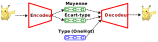
\includegraphics[width=0.48\textwidth]{../img/workshop/AEV.pdf}
	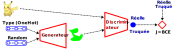
\includegraphics[width=0.48\textwidth]{../img/workshop/GAN.pdf}
	\caption{Architecture d'un générateur des pokémon (a)  basé sur l'auto-encodeur variationnel (b) basé sur les GANs.}
	\label{fig:gen}
\end{figure}


\end{document}
